%%%%%%%%%%%%%%%%%%%%% {{{
%%Options for presentations (in-class) and handouts (e.g. print).
\documentclass[pdf,9pt]{beamer}
% \documentclass[pdf,9pt]{beamer}


%%%%%%%%%%%%%%%%%%%%%%
%Change this for different slides so it appears in bar
\usepackage{authoraftertitle}
\date{Chapter 1. Systems of Linear Equations \\ \S  1-1. Solutions and Elementary Operations}

%%%%%%%%%%%%%%%%%%%%%%
%% Upload common style file
\usepackage{LyryxLAWASlidesStyle}

\begin{document}

%%%%%%%%%%%%%%%%%%%%%%%
%% Title Page and Copyright Common to All Slides

%Title Page
\input frontmatter/titlepage.tex

%LOTS Page
% \input frontmatter/lyryxopentexts.tex

%Copyright Page
% \input frontmatter/copyright.tex

%%%%%%%%%%%%%%%%%%%%%%%%% }}}
%-------------- start slide -------------------------------%{{{ 2
\begin{frame}[fragile]
   \tableofcontents
\end{frame}
%-------------- end slide -------------------------------%}}}
\section[\textcolor{yellow}{}]{\textcolor{yellow}{Solutions of Linear Equations}}
%-------------- start slide -------------------------------%{{{ 4
\frame{
\frametitle{Solutions of Linear Equations}
\pause
\begin{example}
    Find all solutions of the (linear) equation in one variable:
    \[
	ax=b
    \]
\end{example}
\pause
\vfill
\begin{solution}
    \begin{itemize}
	\item If $a \neq 0$, there is  a unique solution $x=b/a$.
	\pause
	\item Else if $a = 0$ and
	\item[] $b\neq 0$, there is  no solution.
	 \pause
     \item[] $b =  0$, there are infinitely many solutions, in fact any $x \in \RR$ is a solution.
    \end{itemize}
    This a complete description of all possible solutions of $ax=b$.
\end{solution}
\pause
\begin{alertblock}{Objective:}
    Can we do the same for linear equations in more variables?
\end{alertblock}
}
%-------------- end slide -------------------------------%}}}
%------------------start slide ---------------------------%{{{ 5
\frame{
\begin{definition}
    A \alert{linear equation} is an expression
    \[ a_1 x_1+a_2 x_2+\dots + a_n x_n = b \]
    where $n\geq 1$, $a_1,\dots, a_n$ are real numbers, \textcolor{lgtblue}{not all of them equal to zero},
    and $b$ is a real number.
    \pause
    \medskip

    A \alert{system of linear equations} is a set of $m\geq 1$ linear equations.
    It is not required that $m=n$.
    \pause
    \medskip

    A \alert{solution} to a system  of $m$ equations in  $n$ variables
     is an $n$-tuple of numbers that satisfy each of the equations.
    \pause
    \medskip

    \alert{Solve a system} means `find \textcolor{lgtblue}{all} solutions to the system'.
\end{definition}
}
%-------------- end slide -------------------------------%}}}
%-------------- start slide  ---------------------------%{{{ 6
\frame{
\begin{example}
    A {\bf system} of {\bf linear equations}:
    \[ \begin{array}{ccccccc}
    x_1 & - & 2x_2 & - & 7x_3 & = & -1 \\
    -x_1 & + & 3x_2 & + & 6x_3 & = & 0
    \end{array}\]
    \pause
    \begin{itemize}
    \item variables: $x_1$, $x_2$, $x_3$.
    \pause
    \item coefficients:
    \[ \begin{array}{ccccccc}
	\alert{1}x_1  & \alert{-} & \alert{2}x_2 & \alert{-} & \alert{7}x_3 & = & -1 \\
	\alert{-1}x_1 & \alert{+} & \alert{3}x_2 & \alert{+} & \alert{6}x_3 & = & 0
    \end{array}\]
    \pause
    \item constant terms:
    \[ \begin{array}{ccccccc}
    x_1 & - & 2x_2 & - & 7x_3 & = & \alert{-1} \\
    -x_1 & + & 3x_2 & + & 6x_3 & = & \alert{0}
    \end{array}\]
    \end{itemize}
\end{example}
}
%-------------- end slide -------------------------------%}}}
%-------------- start slide  ---------------------------%{{{ 7
\frame{
\begin{example}[continued]
    $x_1= \textcolor{coral}{-3}$, $x_2 = \textcolor{coral}{-1}$, $x_3=\textcolor{coral}{0}$ is a \alert{solution} to the system
\[ \begin{array}{ccccccc}
x_1 & - & 2x_2 & - & 7x_3 & = & -1 \\
-x_1 & + & 3x_2 & + & 6x_3 & = & 0
\end{array}\]
\pause
because
\[ \begin{array}{ccccccc}
    (\textcolor{coral}{-3}) & - & 2(\textcolor{coral}{-1}) & - & 7 \cdot \textcolor{coral}{0} & = & -1 \\
    -(\textcolor{coral}{-3}) & + & 3(\textcolor{coral}{-1}) & + & 6\cdot \textcolor{coral}{0} & = & 0.
\end{array}\]
\pause
Another solution to the system is
$x_1= \textcolor{coral}{6}$, $x_2 = \textcolor{coral}{0}$, $x_3=\textcolor{coral}{1}$ (check!).
\pause
\bigskip

However,
$x_1= \textcolor{lgtblue}{-1}$, $x_2 = \textcolor{lgtblue}{0}$, $x_3=\textcolor{lgtblue}{0}$ \alert{is not} a solution to the
system, because
\[ \begin{array}{cccccccc}
    (\textcolor{lgtblue}{-1}) & - & 2\cdot \textcolor{lgtblue}{0} & - & 7\cdot\textcolor{lgtblue}{0} & = & -1 \\
    -(\textcolor{lgtblue}{-1}) & + & 3\cdot \textcolor{lgtblue}{0} & + & 6\cdot \textcolor{lgtblue}{0} & = & 1 & \neq 0
\end{array}\]
\bigskip
\pause

A {\bf solution to the system} must be a solution to {\bf every
equation} in the system.
\vfill
\bigskip

\pause
The system above is \alert{\bf consistent}, meaning that the system
has {\bf at least one} solution.
\end{example}
}
%-------------- end slide -------------------------------%}}}
%-------------- start slide  ---------------------------%{{{ 8
\frame{
\begin{example}[continued]
\[ \begin{array}{ccccccc}
x_1 & + & x_2 & + & x_3 & = & 0 \\
x_1 & + & x_2 & + & x_3 & = & -8
\end{array}\]
is an example of an \alert{\bf inconsistent} system,
meaning that it has no solutions.

\bigskip
\pause

\begin{center}
{\large Why are there no solutions?}
\end{center}
\bigskip

\end{example}
}
%-------------- end slide -------------------------------%}}}
%-------------- start slide  ---------------------------%{{{ 9
\frame{
\begin{example}
Consider the system of linear equations in two variables
\[
    \left\{\begin{array}{c}
    x+y=3 \\ y-x=5
    \end{array}\right.
\]
\pause
A solution to this system is a pair $(x,y)$ satisfying both
equations.
\pause

Since each equation corresponds to a line, a solution to the
system corresponds to a point that lies on both lines, so the
solutions to the system can be found by graphing the two lines and
determining where they intersect.

\pause
\vfill

\begin{center}
    \begin{tikzpicture}[scale=0.9, transform shape]
    \tikzset{>=latex}
    \draw [->] (-2,0) -- (3,0) node [right] {$x$};
    \draw [->] (0,-1) -- (0,3) node [right] {$y$};
    \coordinate (A) at (-1,0);
    \coordinate (B) at (0.6,0);
    \coordinate (C) at (-0.2,0.8);
    \draw [blue] ($(A)!-1cm!(C)$) -- (A) -- (C) -- ($(C)!-2cm!(A)$) node [above] {$y-x=5$};
    \draw [red] ($(B)!-1cm!(C)$) -- (B) -- (C)  node [left] {$(-1,4)$} -- ($(C)!-2cm!(B)$) node [above] {$x+y=3$};
    \filldraw (C) circle (0.05);
    \end{tikzpicture}
\end{center}
\end{example}
}
%-------------- end slide -------------------------------%}}}
%-------------- start slide  ---------------------------%{{{ 10
\frame{

\begin{emptytitle}
Given a system of two equations in two variables,
graphed on the $xy$-coordinate plane, there
are three possibilities:
\end{emptytitle}
\pause
\vfill

\begin{center}
    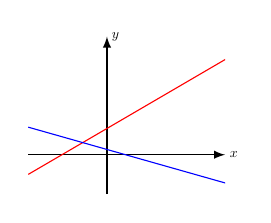
\begin{tikzpicture}[scale=0.5, transform shape]
    \tikzset{>=latex}
    \draw [->] (-2,0) -- (3,0) node [right] {$x$};
    \draw [->] (0,-1) -- (0,3) node [right] {$y$};
    \clip (-2,-1) rectangle (3,3);
    \draw [red] (-2,-0.5) -- (4,3);
    \draw [blue] (-2,0.7) -- (4,-1);
    \end{tikzpicture}
    \hfill
    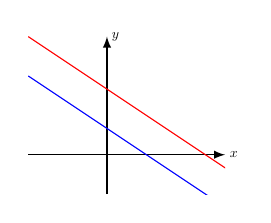
\begin{tikzpicture}[scale=0.5, transform shape]
    \tikzset{>=latex}
    \draw [->] (-2,0) -- (3,0) node [right] {$x$};
    \draw [->] (0,-1) -- (0,3) node [right] {$y$};
    \clip (-2,-1) rectangle (3,3);
    \draw [red] (-2,3) -- (4,-1);
    \draw [blue] (-2,2) -- (4,-2);
    \end{tikzpicture}
    \hfill
    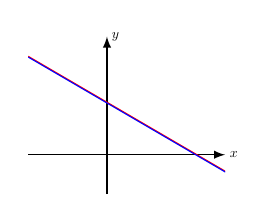
\begin{tikzpicture}[scale=0.5, transform shape]
    \tikzset{>=latex}
    \draw [->] (-2,0) -- (3,0) node [right] {$x$};
    \draw [->] (0,-1) -- (0,3) node [right] {$y$};
    \clip (-2,-1) rectangle (3,3);
    \draw [red] (-2,2.5) -- (4,-1);
    \draw [blue] (-2,2.48) -- (4,-1.02);
    \end{tikzpicture}
\end{center}
\vspace{-10em}
\begin{picture}(4,2.0)
% \put(0,0.5){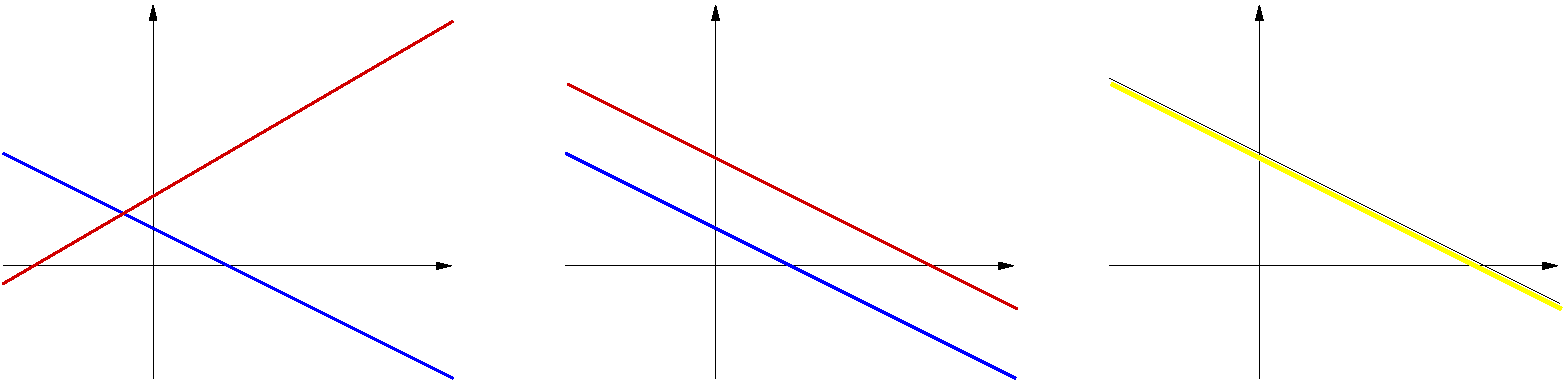
\includegraphics[decodearray={0.2 0.5},scale=0.4]{figures/lines.pdf}}
% \put(0,0.5){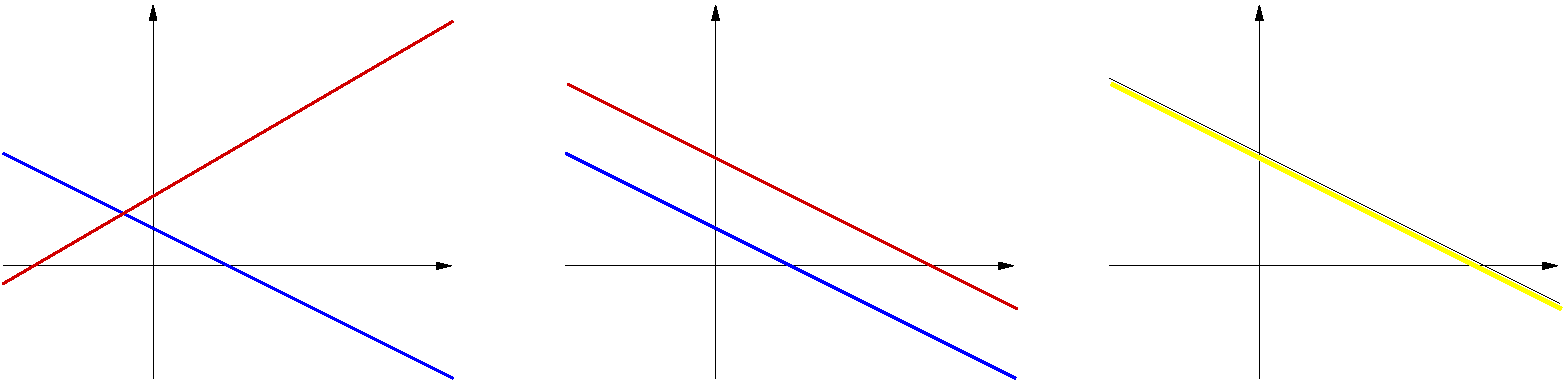
\includegraphics[scale=0.4]{figures/lines.pdf}}
\pause
\put(0.1,0.2){\footnotesize{intersect in one point}}
\pause
\put(0.1,0.0){\textcolor{red}{\footnotesize{consistent}} }
\put(0.1,-0.2){\footnotesize{(unique solution)}}
\pause
\put(1.8,0.2){\footnotesize{parallel but different}}
\pause
\put(1.8,0.0){\textcolor{red}{\footnotesize{inconsistent}} }
\put(1.8,-0.2){\footnotesize{(no solutions)}}
\pause
\put(3.4,0.2){\footnotesize{line are the same}}
\pause
\put(3.4,0.0){\textcolor{red}{\footnotesize{consistent}} }
\put(3.4,-0.2){\footnotesize{(infinitely many solutions)} }
\end{picture}
}
%-------------- end slide -------------------------------%}}}
%-------------- start slide  ---------------------------%{{{ 11
\frame{
\begin{block}{Number of Solutions}\small
For a system of linear equations in {\bf two variables},
exactly one of the following holds:\\[1em]
\pause
\begin{enumerate}
\item the system is \alert{inconsistent};
\pause
\item the system has a \alert{unique} solution, i.e., exactly
one solution;
\pause
\item the system has \alert{infinitely many} solutions.
\end{enumerate}
\pause
\end{block}
\bigskip

\begin{remark}
  We will see in what follows that this generalizes to systems of
linear equations in more than two variables.
\end{remark}
}
%-------------- end slide -------------------------------%}}}
%-------------- start slide -------------------------------%{{{ 12
\frame{
\begin{example}
The system of linear equations in three variables that we saw
earlier
\[ \begin{array}{ccccccc}
x_1 & - & 2x_2 & - & 7x_3 & = & -1 \\
-x_1 & + & 3x_2 & + & 6x_3 & = & 0,
\end{array}\]
has solutions $x_1=-3+9s$, $x_2=-1+s$, $x_3=s$
where $s$ is any real number \alert{(written $s\in\RR$)}.
\pause

Verify this by substituting the expressions for $x_1$, $x_2$,
and $x_3$ into the two equations.

\pause

$s$ is called a \alert{parameter}, and the expression
\[
x_1=-3+9s,\quad x_2=-1+s,\quad x_3=s,\quad\mbox{where } s\in\RR\]

is called the
\alert{general solution} in parametric form.
\end{example}
}
%-------------- end slide -------------------------------%}}}
%-------------- start slide -------------------------------%{{{ 13
\frame{
\begin{problem}
Find all solutions to a system of $m$ linear equations in $n$
variables, i.e., \alert{solve a system of linear equations}.
\end{problem}

\pause
\begin{definition}
Two systems of linear equations are \alert{equivalent} if they
have {\bf exactly the same} solutions.
\end{definition}

\pause
\begin{example}
The two systems of linear equations
\[ \begin{array}{ccccc}
2x & + & y & = & 2 \\
3x &  &  & = & 3
\end{array}
\hspace*{.25in}\quad\text{and}\quad \hspace*{.25in}
\begin{array}{ccccc}
x & + & y & = & 1 \\
&  & y & = & 0
\end{array}\]
are {\bf equivalent} because both systems have the
unique solution $x=1$, $y=0$.
\end{example}
}
%-------------- end slide -------------------------------%}}}
\section[\textcolor{yellow}{}]{\textcolor{yellow}{Elementary Operations}}
%-------------- start slide -------------------------------%{{{ 15
\frame{
\frametitle{Elementary Operations}
\pause
\begin{emptytitle}
Any system of linear equations can be solved by using \alert{\em Elementary Operations}
to transform the system into an equivalent but simpler system from which
the solution can be easily obtained.
\end{emptytitle}
\pause
\vfill

\begin{block}{Three types of Elementary Operations}
\begin{itemize}
    \item[--] {\bf Type I:} Interchange two equations,  \alert{$r_1\leftrightarrow r_2$}.
\pause
\item[--] {\bf Type II:} Multiply an equation by a nonzero number, \alert{$-2r_1$}.
\pause
\item[--]  {\bf Type III:}
Add a multiple of one equation to a different equation, \alert{$3r_3+r_2$}.
\end{itemize}
\end{block}
}
%-------------- end slide -------------------------------%}}}
%-------------- start slide -------------------------------%{{{ 16
\frame{

{
\begin{example}
Consider the system of linear eq's:
$\begin{array}{ccccccc}
    3x_1 & - & 2x_2 & - & 7x_3 & = & -1 \\
    -x_1 & + & 3x_2 & + & 6x_3 & = & 1\\
    2x_1 &   &      & - & x_3  & = & 3
\end{array}$
\pause
\vfill
\begin{enumerate}
\item Interchange first two equations
(Type I ):
\[
\alert{r_1\leftrightarrow r_2}\qquad
\begin{array}{ccccccc}
    -x_1 & + & 3x_2 & + & 6x_3 & = & 1\\
    3x_1 & - & 2x_2 & - & 7x_3 & = & -1 \\
    2x_1 &  &  & - & x_3 & = & 3
\end{array}\]
\pause
\item Multiply first equation by $-2$
(Type II ):
\[ \alert{-2r_1}\qquad
\begin{array}{ccccccc}
    -6x_1 & + & 4x_2 & + & 14x_3 & = & 2 \\
    -x_1 & + & 3x_2 & + & 6x_3 & = & 1\\
    2x_1 &  &  & - & x_3 & = & 3
\end{array}\]
\pause
\item Add 3 time the second equation to the first equation
(Type III ):
\[ \alert{3r_2+r_1}
\qquad
\begin{array}{ccccccc}
    &  & 7x_2 & + & 11x_3 & = & 2 \\
    -x_1 & + & 3x_2 & + & 6x_3 & = & 1\\
    2x_1 &  &  & - & x_3 & = & 3
\end{array}\]
\end{enumerate}
\end{example}
}}
%-------------- end slide -------------------------------%}}}
%-------------- start slide -------------------------------%{{{ 17
\frame{
\begin{theorem}[Elementary Operations and Solutions]
    Suppose that a sequence of elementary operations is performed on a system of linear equations.
    Then the resulting system has the same set of solutions as the original, so the two systems are
    equivalent.
\end{theorem}
\vfill
\pause
\begin{emptytitle}
\alert{As a consequence, performing a sequence of elementary
  operations on a system of linear equations results in an equivalent
  system of linear equations, with the exact same solutions.}
\end{emptytitle}
}
%-------------- end slide -------------------------------%}}}
\section[\textcolor{yellow}{}]{\textcolor{yellow}{The Augmented Matrix}}
%-------------- start slide -------------------------------%{{{ 19
\frame{
\frametitle{The Augmented Matrix}
\pause
\begin{emptytitle}
    Represent a system of linear equations with its
    augmented matrix.
\end{emptytitle}
\begin{example}
    The system of linear equations
    \[ \begin{array}{ccccccc}
	x_1  & - & 2x_2 & - & 7x_3 & = & -1 \\
	-x_1 & + & 3x_2 & + & 6x_3 & = & 0
    \end{array}\]
    is represented by the \alert{augmented matrix}
    \[ \left[\begin{array}{rrr|r}
	1  & -2 & -7 & -1 \\
	-1 & 3  & 6  & 0
    \end{array}\right] \]
    (A \alert{matrix} is a rectangular array of numbers.)
\end{example}
\pause
\vfill
\begin{remark}
    Two other \alert{matrices} associated with a system of
    linear equations are the \textcolor{orange}{coefficient matrix}
    and the \textcolor{blue}{constant matrix}:
    \[ 
	\textcolor{orange}{\left[\begin{array}{rrr} 1 & -2 & -7\\ -1 & 3 & 6 \\ \end{array}\right]},\quad
	\textcolor{blue}{\left[\begin{array}{r} -1 \\ 0 \end{array}\right]}.
    \]
\end{remark}
}
%-------------- end slide -------------------------------%}}}
%-------------- start slide -------------------------------%{{{ 20
\frame{
\begin{emptytitle}
    For convenience, instead of performing {\bf elementary operations} on a system
    of linear equations, perform corresponding
    \alert{elementary row operations} on the
    corresponding {\bf augmented matrix}.
\end{emptytitle}
\vfill
\pause
\begin{emptytitle}
    {\bf Type I:} Interchange two rows.
\end{emptytitle}
\begin{example}
    Interchange rows 1 and 3.
    \[
    \left[\begin{array}{rrrr|r}
    \textcolor{blue}{2} & \textcolor{blue}{-1} & \textcolor{blue}{0} & \textcolor{blue}{5} & \textcolor{blue}{-3 }\\
    -2 & 0 & 3 & 3 & -1 \\
    \textcolor{red}{0} & \textcolor{red}{5} & \textcolor{red}{-6} & \textcolor{red}{1} & \textcolor{red}{0} \\
    1 & -4 & 2 & 2 & 2
    \end{array}\right]
    \onslide<+->
    \stackrel{r_1\leftrightarrow r_3}{\longrightarrow}
    \left[\begin{array}{rrrr|r}
    \textcolor{red}{0} & \textcolor{red}{5} & \textcolor{red}{-6} & \textcolor{red}{1} & \textcolor{red}{0} \\
    -2 & 0 & 3 & 3 & -1 \\
    \textcolor{blue}{2} & \textcolor{blue}{-1} & \textcolor{blue}{0} & \textcolor{blue}{5} & \textcolor{blue}{-3} \\
    1 & -4 & 2 & 2 & 2
    \end{array}\right]
    \]
\end{example}
}
%-------------- end slide -------------------------------%}}}
%-------------- start slide -------------------------------%{{{ 21
\frame{
\begin{emptytitle}
    {\bf Type II:} Multiply a row by a nonzero number.
\end{emptytitle}
\begin{example}
    Multiply row 4 by 2.
    \[
    \left[\begin{array}{rrrr|r}
	2                   & -1                   & 0                   & 5                   & -3 \\
	-2                  & 0                    & 3                   & 3                   & -1 \\
	0                   & 5                    & -6                  & 1                   & 0  \\
	\textcolor{blue}{1} & \textcolor{blue}{-4} & \textcolor{blue}{2} & \textcolor{blue}{2} & \textcolor{blue}{2}
    \end{array}\right]
    \onslide<+->
    \stackrel{2r_4}{\longrightarrow}
    \left[\begin{array}{rrrr|r}
	2                   & -1                   & 0                   & 5                   & -3 \\
	-2                  & 0                    & 3                   & 3                   & -1 \\
	0                   & 5                    & -6                  & 1                   & 0  \\
	\textcolor{blue}{2} & \textcolor{blue}{-8} & \textcolor{blue}{4} & \textcolor{blue}{4} & \textcolor{blue}{4}
    \end{array}\right]
    \]
\end{example}
}
%-------------- end slide -------------------------------%}}}
%-------------- start slide -------------------------------%{{{ 22
\frame{
\begin{emptytitle}
{\bf Type III:} Add a multiple of one row to a different row.
\end{emptytitle}
\begin{example}
    Add 2 times row 4 to row 2.
    \[
    \left[\begin{array}{rrrr|r}
	2                    & -1                  & 0                   & 5                   & -3                   \\
	\textcolor{blue}{-2} & \textcolor{blue}{0} & \textcolor{blue}{3} & \textcolor{blue}{3} & \textcolor{blue}{-1} \\
	0                    & 5                   & -6                  & 1                   & 0                    \\
	1                    & -4                  & 2                   & 2                   & 2
    \end{array}\right]
    \onslide<+->
    \stackrel{2r_4+r_2}{\longrightarrow}
    \left[\begin{array}{rrrr|r}
	2                   & -1                   & 0                   & 5                   & -3                   \\
	\textcolor{blue}{0} & \textcolor{blue}{-8} & \textcolor{blue}{7} & \textcolor{blue}{7} & \textcolor{blue}{3 } \\
	0                   & 5                    & -6                  & 1                   & 0                    \\
	1                   & -4                   & 2                   & 2                   & 2
    \end{array}\right]
    \]
\end{example}
}
%-------------- end slide -------------------------------%}}}
%-------------- start slide -------------------------------%{{{ 23
\frame{
\begin{definition}
    Two matrices $A$ and $B$ are \alert{row equivalent} (or simply
    equivalent) if one can be obtained from the other by a
    sequence of \alert{elementary row operations}.
\end{definition}
\vfill
\pause
\begin{problem}
    Prove that  $A$  can be obtained from $B$  by a
    sequence of elementary row operations if and only if $B$ can be
    obtained from $A$ by a sequence of elementary row operations.

    Prove that row equivalence is an equivalence relation.
\end{problem}
}
%-------------- end slide -------------------------------%}}}
\section[\textcolor{yellow}{}]{\textcolor{yellow}{Solving a System using Back Substitution}}
%-------------- start slide -------------------------------%{{{ 25
\frame{
\frametitle{Solving a System using Back Substitution}
\pause
\begin{problem}
    Solve the system using back substitution
    \[
	\begin{array}{c}
	    2x+y = 4 \\
	    x-3y = 1
	\end{array}
    \]
\end{problem}
\pause
\vfill
\begin{solution}
    Add $(-2)$ times the second equation to the first equation.
    \[
    \begin{array}{c}
    2x+y \alert{+ (-2)x - (-2)(3)y}= 4 \alert{+ (-2)1}\\
    x - 3y = 1
    \end{array}
    \]
    \pause
    The result is an equivalent system
    \[
    \begin{array}{c}
    7 y = 2 \\
    x - 3y = 1
    \end{array}
    \]
\end{solution}
}
%-------------- end slide -------------------------------%}}}
%-------------- start slide -------------------------------%{{{ 26
\frame{
\begin{solution}[continued]
    The first equation of the system,
    \[
	\alert{7y=2}
    \]
    can be rearranged to give us
    \[
	\alert{y= \frac{2}{7}}.
    \]
    \pause
    Substituting $y=\frac{2}{7}$ into second equation:
    \[
	x - 3y = x - 3 \left(\alert{\frac{2}{7}}\right)= 1,
    \]
    \pause
    and simplifying, gives us
    \[
	x = 1 + \frac{6}{7} = \frac{13}{7}.
    \]
    \pause
    Therefore, the solution is $x={13}/{7}, y = {2}/{7}$.
    \pause
    \bigskip

    The method illustrated in this example is called \alert{back substitution.}
    \myQED
\end{solution}
\vfill
\pause
\begin{emptytitle}
    We shall describe an \textcolor{lgtblue}{algorithm} for solving any given system of linear equations.
\end{emptytitle}
}
%-------------- end slide -------------------------------%}}}
\end{document}
